\documentclass[10pt,a4]{article}
\usepackage[english]{babel}
\usepackage[utf8x]{inputenc}
\usepackage{amsmath}
\usepackage{graphicx}
\usepackage[colorinlistoftodos]{todonotes}
\usepackage{hyperref}
\usepackage{geometry}
\geometry{top=3cm,left=2cm,right=2cm,bottom=3cm}
\usepackage[scaled]{helvet}
\usepackage[T1]{fontenc}
\usepackage{float}
\renewcommand\familydefault{\sfdefault}


\author{Apollonio Marco, Bossi Giacomo}
\date{\today}
\title{Proof of concept for integrating TORCS within a DDS environment}



\begin{document}
\maketitle
\tableofcontents


\section{Project data}

\begin{itemize}
  \item
        Project supervisor(s): Prof. Vittorio Zaccaria

  \item
        Describe in this table the group that is delivering this project:

        \begin{center}
          \begin{tabular}{lll}
            Last and first name & Person code & Email address                   \\
            \hline
            Marco Apollonio     & 10764083    & marco2.apollonio@mail.polimi.it \\
            Giacomo Bossi       & 10766073    & giacomo3.bossi@mail.polimi.it
          \end{tabular}
        \end{center}

  \item
        Describe here how development tasks have been subdivided among members
        of the group, e.g.:

        \begin{itemize}
          \item Bossi configured the Docker environment to simplify the development process.
          \item Apollonio worked on the integration of the OpenDDS library within the TORCS simulator.
          \item ...
        \end{itemize}

  \item Links to the project source code; Put here, if available, links to public repos hosting your project

\end{itemize}


\section{Project description}

\textbf{2 pages max please}

\begin{itemize}
  \item What is your project about?
  \item Why it is important for the AOS course?
\end{itemize}

\subsection{Introduction}

\par The project aims to integrate the TORCS simulator within a DDS environment, in order to test the real time
communication between a ECU, being it a real one or a simulated one, and the TORCS simulator.
\par The project is divided in two Proof of Concepts, each one with a specific goal to achieve:
\begin{itemize}
  \item The first Proof of Concept aims to send the steering commands from the ECU to the TORCS simulator using The
        Vehicle Signal Specification (VSS) standard. One modification done to the VSS standard is the usage of the steering
        wheel as an actuator instead of being a sensor.
  \item The second Proof of Concept aims to create a torque vectoring algorithm on the ECU so that it receives as an input
        the yaw rate and the lateral acceleration of the car from the simulator and the angle of the steering wheel from the steering
        wheel. The ECU will then calculate the torque to be applied to each wheel and send it to the simulator.
        All this communication will be done using the DDS environment, without the usage of the VSS standard.
\end{itemize}

\subsection{Design and implementation}


\par For each proof of concept we developed a specific bot that need to be selected in the TORCS simulator.
The bot will have the Publisher and Subscriber functionalities to communicate with the DDS environment based on
the requirement needed to verify the proof of concept.


\subsubsection{Design of First Proof of Concept}

\par For the first Proof Of Concept we decided to create two topics in the DDS environment,
using the VSS standard for the steering commands:
\begin{itemize}
  \item SteeringInformation: it's used to send the steering commands to the TORCS simulator.
        % decide if second topic is really necessary
  \item WheelInformation: it's used to send the wheels rotation information from the TORCS simulator to the ECU.
\end{itemize}

\par The ECU will have a Publisher for the SteeringInformation topic and a Subscriber for the WheelInformation topic.
The TORCS simulator will have a Subscriber for the SteeringInformation topic and a Publisher for the WheelInformation topic.

\begin{figure}[H]
  \centering
  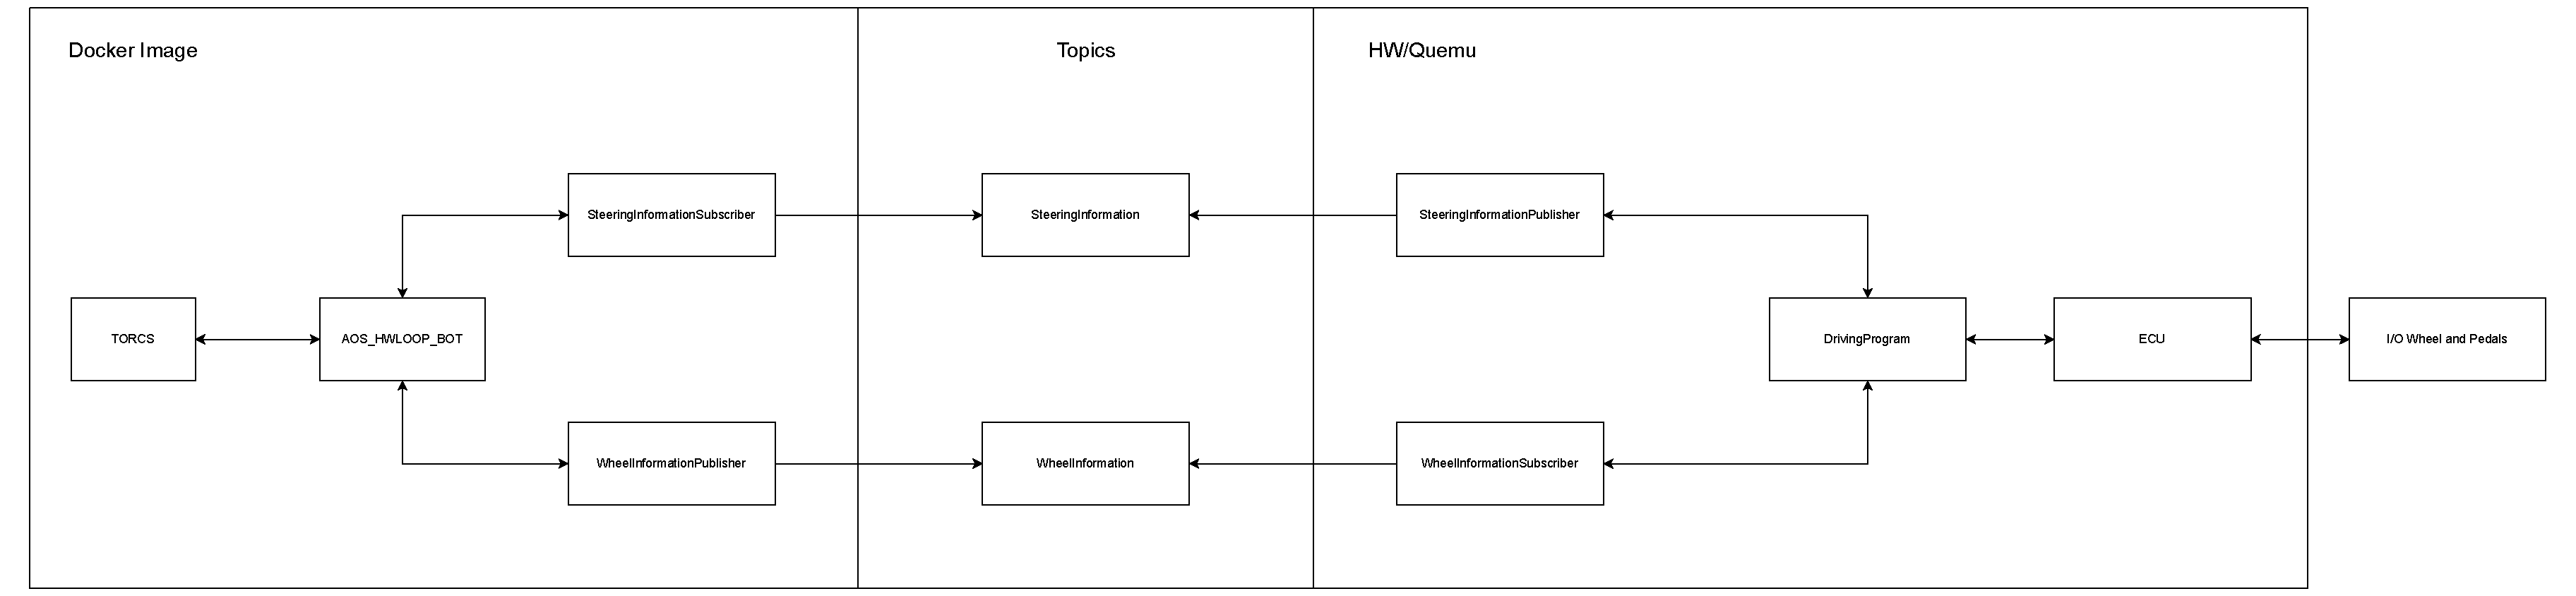
\includegraphics[width=1.0\textwidth]{Images/Schematization_PoC_1.pdf}
  \caption{Schematization of the first proof of concept}
  \label{fig:schematization-poc-1}
\end{figure}

\subsubsection{Design of Second Proof of Concept}


\section{Project outcomes}

\subsection{Concrete outcomes}
Describe the artifacts you've produced, if possible by linking to repo commits.
For those who choose to work on an open source project, please put here the
\textbf{URL to your final pull request}.

Those that have chosen to present a paper can include a link to the slides.

\subsection{Learning outcomes}

What was the most important thing all the members have learned while
developing this part of the project, what questions remained unanswered,
how you will use what you've learned in your everyday life?
Please also indicate which tools you learned to use.

Examples:

\begin{itemize}
  \item Foo learned to write multithreaded applications, he's probably going to
        create his own startup with what she has learned. She also learned how to
        debug with gdb.
  \item Bar learned how to interact with the open source community, politely
        answering to code reviews and issuing pull requests through Git.
\end{itemize}

\subsection{Existing knowledge}
What courses you have followed (not only AOS) did help you in doing this project
and why? Do you have any suggestions on improving the AOS course with topics
that would have made it easier for you?

\subsection{Problems encountered}
What were the most important problems and issues you encountered? Did you ever
encountered them before?

\begin{itemize}
  \item Foo encountered a problem with some critical sections. He ended up
        rewriting existing lock implementation.
\end{itemize}

\section{Honor Pledge}
 (\textbf{This part cannot be modified and it is mandatory to sign it})

I/We pledge that this work was fully and wholly completed within the criteria
established for academic integrity by Politecnico di Milano (Code of Ethics and
Conduct) and represents my/our original production, unless otherwise cited.

I/We also understand that this project, if successfully graded,  will fulfill part B requirement of the
Advanced Operating System course and that it will be considered valid up until
the AOS exam of Sept. 2022.

\begin{flushright}
  Group Students' signatures
\end{flushright}


\end{document}